\documentclass{article}
\usepackage{CJKutf8}
\usepackage[dvipdfmx,unicode=true,colorlinks=false,pdfborder={0 0 0}]{hyperref}
\usepackage{indentfirst}
\usepackage[dvipdfmx]{graphicx}
\begin{document}
\begin{CJK}{UTF8}{gbsn}
\title{Zby's Printing Service\\石头、剪子、布 打印店\\技术摘要 v0.0.1}
\author{北京大学附属中学 2014 届 5 单元 3 班 张博洋}
\date{2012 年 6 月}
\maketitle
\thispagestyle{empty}
\newpage

\renewcommand\contentsname{目\quad 录}
\renewcommand\figurename{图}
\renewcommand\tablename{表}
\tableofcontents
\thispagestyle{empty}
\newpage
\pagenumbering{arabic}
\CJKindent

\section{自动网络打印分析与计划系统}
	\subsection{综述}
		“自动网络打印分析与计划系统”由网页服务器和后端 IPP 服务器组成。网页服务器采用 LAMP(Linux + Apache + MySQL + PHP) 架构,IPP 服务器采用 CUPS,并使用使用 Ubuntu 12.04 Server LTS 作为系统。该系统完成的任务如下:
		\begin{itemize}
			\item{处理用户提交的打印任务,分析出页面黑色部分面积,自动计算出打印费用。}
			\item{保存用户的账户信息(包括账户密码,用户余额等)。}
			\item{处理用户的注册、登录、充值请求。}
			\item{为用户提供详细的帮助。}
		\end{itemize}
		
	\subsection{网页平台}
		网页平台全面采用 AJAX 技术,所有功能全部在一个网页中完成。网站分为以下模块:
		\begin{itemize}
			\item{作业控制模块:该模块主要提供用户对自己作业的浏览与控制功能。在这个模块,用户可以确认、取消、查看作业状态。}
			\item{用户账户模块:该模块提供查询余额、查询详单、充值、修改密码等功能。}
			\item{系统公告模块:该模块可以显示系统公告。}
			\item{注册登录模块:该模块提供用户注册与登录验证等功能。}
		\end{itemize}
	
	\subsection{工作原理}
		用户从终端(可以是 Windows, Mac OS, Linux, iOS 等)使用 IPP 协议将任务传送到 CUPS 服务器中,然后服务器接到任务后启动程序分析这个任务中页面的黑色部分面积,计算出价格,存入后台数据库中。之后用户访问网页平台,在网页平台浏览任务分析结果,并确认任务,服务器收到确认信息后,将任务发送到“打印机控制系统”,由该系统控制打印机打印这个任务。

	\subsection{网页截图}
		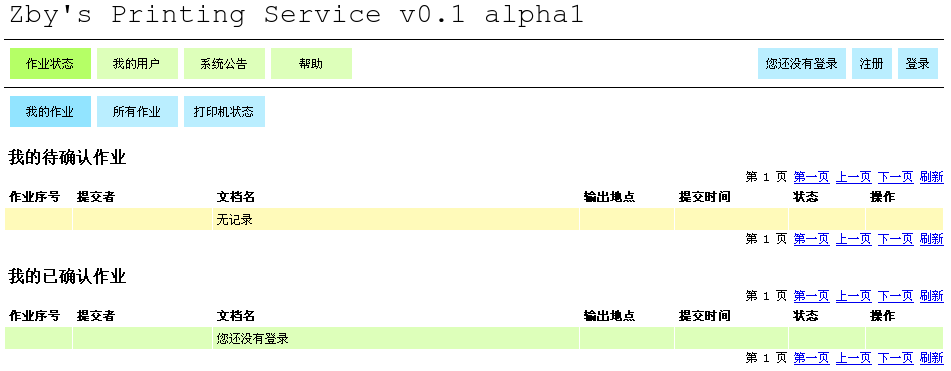
\includegraphics[width=\textwidth]{screenshot.png}
\newpage

\section{打印机控制系统}
	\subsection{综述}
		“打印机控制系统”是一个抽象的系统,它只需要接受从“自动网络打印分析与计划系统”发来的任务并打印即可,所以它根据不同需要有多种不同实现。由于时间关系,目前这套系统还没有实现,计划于 2012 暑假完成。
	\subsection{基于 CUPS 的实现}
		由于“自动网络打印分析与计划系统”使用了 CUPS 系统,那么最好的方案也是在“打印机控制系统”中采用 CUPS 系统,这样可以取得最大的兼容性。
	\subsection{基于 Microsoft Windows Server 的实现}
		由于某些打印机驱动程序只支持 Microsoft Windows 系统,所以需要使用 Microsoft Windows 自带的 IIS 服务来实现。
\newpage

\section{附录:苹果公司的 AirPrint 原理}
	AirPrint 协议是基于标准 IPP 协议的\cite{airprint},只不过添加了一些其他的 TXT 记录而已,这些记录如下:
	\begin{verbatim}
	pdl=application/pdf,image/jpeg,image/urf
	URF=none
	\end{verbatim}
	当打印机有密码保护时,还会多出这一条记录:
	\begin{verbatim}
	air=username,password
	\end{verbatim}
	iPhone, iPod Touch, iPad 等通过 AirPrint 打印的流程如下。
	\subsection{查找服务器}
		用户手中的设备会通过 Bonjour 服务或当前 DNS 服务器发现局域网中的打印机。由于打印店只需通过 DNS 发布自己,这里只讨论 DNS 方法。\\
		当设备没有设置搜索域时,设备会将向当前的 DNS 服务器查询以下 PTR 记录。
		\begin{verbatim}
		_universal._sub._ipps._tcp.localhost
		\end{verbatim}
		当查询到之后,设备会用该记录的返回结果继续查询,例如第一次查询结果为:
		\begin{verbatim}
		zbyprinting._printer._tcp.localhost
		\end{verbatim}
		设备就会向 DNS 服务器查询这个主机的 TXT 与 SRV 记录,TXT 记录用来描述打印机,SRV 记录用来指示打印服务器的位置。
	\subsection{发送打印任务}
		查找到服务器后,设备会使用标准 IPP 协议试图连接打印服务器,并将打印作业发送到服务器上。
\newpage
\addcontentsline{toc}{section}{参考文献}
\renewcommand\refname{\hfil 参~考~文~献}
\begin{thebibliography}{1}
	\bibitem{airprint}\textsl{AirPrint and Linux}, Ryan Finnie, \textsl{http://www.finnie.org/2010/11/13/airprint-and-linux/}
\end{thebibliography}

\newpage
\end{CJK}
\end{document}
